I dette kapitel anvendes \cite[s. 1-111]{olofsson2005probability} og \cite[s. 24-32]{oxford}. 

For at kunne definere og analysere \textit{Markov-kæder} skal der først introduceres nogle basale begreber om \textit{sandsynlighed}. Disse begreber defineres i dette kapitel. 

\section{Introduktion}
%To primære fortolkninger af sandsynlighed er, at en sandsynlighed er grænsen for den relative frekvens eller en vis grad af tro. Ud over disse to fortolkninger er det muligt at formulere en matematisk definition af, hvad sandsynlighed er.


%

%Hvis man kaster en mønt vil de fleste mene at der er $50\%$ chance for at den lander på krone. Derudover kan man kaste mønten mange gange og se at ca halvdelen af gangene man kaster mønten rammer den krone. I dette afsnit vil en matematiske definition på sandsynlighed præsenteres, og det vil være denne definition som fremadrettet vil blive anvendt.

%I dette projekt defineres sandsynlighed aksiomatisk
%Endeligt, er det muligt at formulere en matematisk definition af, hvad sandsynlighed er.


%Derudover bliver ordet sandsynlighed brugt om hvad en person tror vil være 



%For at kunne beskrive en sandsynlighed matematisk skal begreber som \textit{tilfældighed}, \textit{udfaldsrum}, \textit{hændelser} og \textit{hændelsesrum} først beskrives.

Noget kaldes \textit{tilfældigt}, hvis det ikke er muligt at forudse udfaldet. Hvis der udføres et eksperiment, hvor udfaldet er tilfældigt, kaldes det et \textit{tilfældigt eksperiment}, $\E$. Et eksempel på et tilfældigt eksperiment er et terningkast, hvor det ikke er sikkert, hvorvidt udfaldet er $1, 2, \dots$ eller $6$. %%For et tilfældigt eksperiment defineres begreberne, \textit{udfaldsrum}, \textit{hændelser} og \textit{hændelsesrum} som følgende

Mængden af mulige udfald i et tilfældigt eksperiment, $\E$, kaldes et \textit{udfaldsrum} og noteres $\Omega$. Et udfaldsrum kan bestå af en \textit{endelig}, \textit{tællelig uendelig} eller en \textit{ikke-tællelig uendelig} mængde af udfald. Hvis udfaldene er adskilt i punkter, eksempelvis $\{1,2,3, \dots\}$, er det et tælleligt udfaldsrum, og hvis det derimod er et kontinuum af punkter, er det ikke-tælleligt. Eksempelvis er udfaldsrummet $[0, 10]$ ikke-tælleligt.

Ud fra udfaldsrummet defineres begrebet \textit{hændelsesrum} og \textit{hændelse} som følgende.

\begin{defn}\textbf{Hændelsesrum}
\newline
    Mængden af delmængder af udfaldsrummet, $\Omega$, kaldes et hændelsesrum og noteres $\mathcal{F}$, hvis
    \begin{enumerate}
        \item $\F$ er ikke-tom,
        \item $A\in\F$, så er $A^c=\Omega\backslash A \in \mathcal{F}$,
        \item $A_1, A_2,\dots\in \F$, så er $\displaystyle \bigcup_{k=1}^\infty A_k\in\F$.
    \end{enumerate}
Elementerne, $A\in \F$, kaldes for hændelser.
\end{defn}

Hvis der for to hændelser $A$ og $B$ gælder, at $A \cap B = \varnothing$, kaldes hændelserne for \textit{disjunkte}.

Det er ud fra ovenstående muligt at definere et \textit{sandsynlighedsmål}.

\begin{defn}\textbf{Sandsynlighedsregningens aksiomer} \label{def:sandsynlighedsregningens_grundsætninger}%Ny definition
\newline
Lad $\Omega$ være et udfaldsrum, $\F$ et hændelsesrum og $A$ en hændelse. En funktion,\\ $P: \F \to [0,1]$, kaldes et sandsynlighedsmål på $(\Omega, \F)$, hvis
\begin{enumerate}
    \item $0 \leq P(A) \leq 1$,
    \item $P(\Omega) = 1$ og $P(\emptyset)=0$,
    \item $(A_1, A_2, \ldots) $ er en sekvens af parvise disjunkte hændelser, altså $A_i \cap A_j = \emptyset$ for $i \neq j$, så er
    \begin{align*}
        P\left(\bigcup_{k=1}^\infty A_k \right) = \sum_{k=1}^\infty P(A_k).
    \end{align*}
\end{enumerate}
\end{defn}

Jævnfør punkt 3 i \autoref{def:sandsynlighedsregningens_grundsætninger} følger det, at
\begin{align*}
    P\left(\bigcup_{k=1}^n A_k \right) = \sum_{k=1}^n P(A_k),
\end{align*}
ved at lade $A_k = \emptyset$ for $k > n$.

Ud fra udfaldsrum, hændelsesrum og sandsynlighedsmål defineres \textit{sandsynlighedsrum} som følgende

\begin{minipage}\textwidth
\begin{defn}\textbf{Sandsynlighedsrum} \label{def:sandsynlighedsrum}\\
    Lad $\Omega$ være et udfaldsrum, $\mathcal{F}$ et hændelsesrum og $P$ et sandsynlighedsmål på $(\Omega, \F)$. Så er sandsynlighedsrummet givet ved triplen, $(\Omega, \F, P)$. 
\end{defn}
\end{minipage}







\section{Betinget sandsynlighed}
Hvis man har ekstra information om en given hændelse, så vil udfaldsrummet indskrænkes - mere formelt:\\
\begin{minipage}\textwidth
\begin{defn}\textbf{Betinget sandsynlighed} %Ny definition
\newline
Lad $B$ være en hændelse sådan at $P(B)>0$. Den \textit{betingede sandsynlighed} af $A$ givet $B$ er defineret som
\begin{align*}
      \displaystyle P(A|B)=\frac{P(A\cap B)}{P(B)}
\end{align*}
\end{defn}
\end{minipage}

\subsection{Uafhængige hændelser}
Hvis to hændelser, $A$ og $B$, er \textit{uafhængige}, vil en betingelse $B$ ikke påvirke sandsynligheden for $A$. Med andre ord, så er den betingede og ubetingede sandsynlighed den samme. Dette har konsekvensen, at $P(A)=P(A|B)\Leftrightarrow P(A\cap B)=P(A)P(B)$. Faktisk kan dette generaliseres til følgende definition:\\
\begin{minipage}\textwidth
\begin{defn}\textbf{Uafhængighed} %Ny definition
\newline
Hændelserne, $A_1,A_2,\dots$ siges at være uafhængige hvis
\begin{align*}
    P(A_{i_1}\cap A_{i_2}\cap\cdots\cap A_{i_k})=P(A_{i_1})P(A_{i_2})\cdots P(A_{i_k})
\end{align*}
for alle følger af heltal, $i_1<i_2<\cdots<i_k, k=2,3,\dots$.
Hvis de ikke er uafhængige er \textit{afhængige}.
\end{defn}
\end{minipage}
\subsection{Total sandsynlighed}
I tilfælde af, at sandsynligheden for en given hændelse er svær at bestemme direkte kan det i nogle tilfælde være hensigtsmæssigt at opdele problemet i termer af betinget sandsynlighed.



\begin{minipage}\textwidth
\begin{thmx} \textbf{Loven om Total Sandsynlighed} \label{sæt:loven_om_total_sandsynlighed} %Ny sætning
\newline
Lad $B_1,B_2,\dots$ være en følge af hændelser, sådan at
\begin{enumerate}[label=(\textbf{\alph*})]
\item $P(B_k)>0$ for $k=1,2,\dots$
\item $B_i$ og $B_j$ er disjunkte når $i\neq j$
\item $S=\bigcup_{k=1}^\infty B_k$
\end{enumerate}
Så for enhver hændelse, $A$ gælder der, at
\begin{align*}
    P(A)=\sum_{k=1}^\infty P(A|B_k)P(B_k)
\end{align*}
\end{thmx}
\end{minipage}
\begin{bev} \textbf{} %Nyt bevis
\newline
Bemærk, at
\begin{align*}
    A=A\cap S=\bigcup_{k=1}^\infty(A\cap B_k)
\end{align*}
i henhold til den distributive lov for uendelige foreningsmængder (se Bilag \ref{Distributive love}). 
Eftersom $A\cap B_1,A\cap B_2,\dots$ er parvis disjunkte fås
\begin{align*}
    P(A)=\sum_{k=1}^\infty P(A\cap B_k)=\sum_{k=1}^\infty P(A|B_k)P(B_k)
\end{align*}
\end{bev}
%By virtue of Proposition 1.2, we realize that the law of total probability is also true for a finite union of events
%Hvis mængden af hændelser er endelig og givet ved $n$, kan man konstruere en uendelig følge af hændelser, sådan at P(\bigcup_{k=n}^\infty B_k)=0.
For $n=2$ gælder der, at hvis $B_1=B$, så følger det at $B_2=B^c$ og følgende korollar fås.
\begin{minipage}\textwidth
\begin{kor} \textbf{} %Nyt korollar
\newline
Hvis $0<P(B)<1$, så er
\begin{align*}
    P(A)=P(A|B)P(B)+P(A|B^c)P(B^c)
\end{align*}
\end{kor}
\end{minipage}
\iffalse
Idét foreningsmængder er kommutative, gælder der, at
$$P(B_j|A)P(A)=P(A|B_j)P(B_j)$$
som må betyde, at
$$P(B_j|A)=\frac{P(A|B_j)P(B_j)}{P(A)}$$

Dette leder op til følgende proposition:\\
\begin{minipage}\textwidth
\begin{pro} \textbf{(Bayes' Formel).} %Ny proposition
\newline
Med samme antagelser som i Loven om Total Sandsynlighed og hvis $P(A)>0$, så gælder der for enhver hændelse, $B_j$, at
\begin{align*}
    P(B_j|A)=\frac{P(A|B_j)P(B_j)}{\sum_{k=1}^\infty P(A|B_k)P(B_k)}
\end{align*}
\end{pro}
\end{minipage}
\begin{bev}
Beviset følger af foregående udregninger.
\end{bev}

Analogt, følger denne korrollar:\\
\begin{minipage}\textwidth
\begin{kor} \textbf{} %Nyt korollar
\newline
Hvis $0<P(B)<1$ og $P(A)>0$, så er
\begin{align*}
    P(B|A)=\frac{P(A|B)P(B)}{P(A|B)P(B)+P(A|B^c)P(B^c)}
\end{align*}
\end{kor}
\end{minipage}
\fi

\section{Tilfældige variabler}

$S = \{1,2,3\}$
$\Sigma = \{\emptyset, \{ 1\}, \{ 2\}, \{ 3\},  \{ 1, 2\}, \{ 2,3 \}, \{ 1,3\}, S\}$
\pagebreak
Tilfældig variabel:\\
En tilfældig variabel på $(S,\Sigma, P)$ er en funktion $X:S\to \R$ således at:\\
$\forall x\in \R : \{s \in S: X(s)\leq x\} \in \Sigma$

Tilfældig diskret variabel:\\
Billedet er en tællelig delmængde af $\R$\\
$\forall x\in \R : \{s \in S: X(s) = x\} \in \Sigma$


\begin{minipage}\textwidth
\begin{defn}\textbf{Hændelsesrum}\\
    Lad $S$ være et udfaldsrum for et eksperiment $\E$.
    
    Hændelsesrummet er givet ved potensmængden
    $\Sigma = \{A:A\subseteq S\}$.
\end{defn}
\end{minipage}
derved er hændelsesmængden givet ud fra alle mulige hændelser

\begin{minipage}\textwidth
\begin{defn}\textbf{Sandsynlighedsrum}\\
    Lad $S$ være et udfaldsrum, $A$ et hændelsesrum til $S$ og $P$ et sandsynlighedsmål over hændelsesrummet. 
    
    Så er sandsynlighedsrummet givet ved tretupelen $(S, \Sigma, P)$ for et eksperiment, $\E$.
\end{defn}
\end{minipage}


% \begin{minipage}\textwidth
% \begin{defn}\textbf{Tilfældig variabel} %Ny definition
% \newline
% En tilfældig variabel er en variabel, $x\in \R$, der får sin værdi fra et tilfældigt eksperiment.
% \end{defn}
% \end{minipage}

% \begin{minipage}\textwidth
% \begin{defn}\textbf{Tilfældig variabel} %Ny definition
% \newline
% Lad $\E$ være et eksperiment med sandsynlighedsrummet $(S, \Sigma, P)$.

% Så er en tilfældig variabel en funktion på sandsynlighedsrummet $X:S\to \R$.


% \end{defn}
% \end{minipage}


En tilfældig variabel, $X$, er en reel variabel som får sin værdi fra et eksperiment. 
Tilfældige variabler kan udtrykkes som reelle funktioner, der tildeler reelle værdier til de mulige udfald af eksperimentet.

%En tilfældig variabel er en variabel, $X$, der først tildeles en værdi efter eksperimentet er udført. 
Da $X$ først antager en værdi efter eksperimentet, er det kun muligt at beskrive billedet af $X$, som er mængden af mulige værdier $X$ kan antage, samt de  tilhørende sandsynligheder. Billedet af $X$ betegnes $range(X)$ og de tilhørende sandsynligheder kaldes for \textit{fordelingen} af $X$.

% Før eksperimentet er det muligt at beskrive mængden af mulige værdier, $range(X)$, og de tilhørende sandsynligheder, \textit{fordelingen} af $X$.
% Det betyder, at det er muligt at beskrive billedet af $X$, men ikke hvilken værdi $X$ antager.

\begin{minipage}\textwidth
\begin{defn}\label{def:Diskret_tilfældig_variabel}\textbf{Diskret tilfældig variabel} %Ny definition
\newline
Lad $(S, \Sigma, P)$ være et sandsynlighedsrum. En diskret tilfældig variabel $X$ er en reel funktion på sandsynlighedsrummet $X:S\to \R$ således, at
%
\begin{align}
    &\text{$Range(X)$ er en tællelig delmængde af $\R$ } \quad \text{og}\label{eq:def_diskretitet_betingelsen}\\
    &\forall x\in \R: \{s\in S: X(s)=x\}\in % S\cup \{\emptyset\} \subseteq 
    \Sigma\label{eq:def_tilfældig_variabel}
\end{align}

\end{defn}
\end{minipage}


At en funktion er diskret betyder, at dens billede er tællelig. 
I \autoref{def:Diskret_tilfældig_variabel} er
\eqref{eq:def_diskretitet_betingelsen} betingelsen, der sikrer, at $X$ er en diskret funktion.

%Dette betyder, at \eqref{eq:def_diskretitet_betingelsen} er betingelsen, der sikrer, at $X$ er diskret.  


% Betingelse (2,2):\\ 
% Da den værdi en diskret variabel $X$ antager, ikke kan forudsiges, 



% En diskret variabel $X$ antager værdier fra $\R$, men man kan ikke forudsige værdien af $X$ før eksperimentet er udført.

% Af denne grund, vil vi finde sandsynligheden for at $X$ er en given værdi $x$. 

%Det bemærkes, at $X$ antager værdien $x$ hvis og kun hvis resultatet af eksperimentet ligger i delmængden som afbilledes over i $x$ - altså delmængden $X^{-1}(x) = \{s\in S: X(s)=x\}$. Betingelse (2,2) postulerer at alle sådanne delmængder er hændelser, og da alle kombinationer af hændelser er i $\Sigma$, kan en tilsvarende sandsynlighed findes.

Det bemærkes, at $X$ antager værdien $x$ hvis og kun hvis resultatet af eksperimentet, $\E$, ligger i en delmængde af $S$ som afbilledes over i $x$. Derved ligger resultatet af $\E$ i delmængden $X^{-1}(x) = \{s\in S: X(s)=x\} \subseteq S\cup \{\emptyset\}$, hvor det bemærkes, at  $X^{-1}(x)\subseteq S\cup \{\emptyset\} \subseteq \Sigma$.
Betingelse \eqref{eq:def_tilfældig_variabel} gør derfor, at alle sådanne delmængder er elementer af hændelsesrummet, $\Sigma$, og derfor har en tilsvarende sandsynlighed, $P$.

Da den diskret tilfældige variabel kan antage flere værdier, defineres en funktion, der bestemmer sandsynligheden for hvert udfald af den diskret tilfældige variabel.

Fremadrettet vil $\{s\in S: X(s)=x\}$ blive betegnet $\{X=x\}$.

\begin{minipage}\textwidth
\begin{defn}\label{def:Frekvensfunktionen}\textbf{Frekvensfunktionen} %Ny definition
\newline
    Lad $X$ være en diskret tilfældig variabel. % med range $\{x_k| k\in N \subseteq \N\}$. 
    Funktionen $p_X:\R\to [0,1]$ defineret ved
%    
    $$ p_X(x) = P(X = x)$$
%    
    kaldes for \textit{frekvensfunktionen} eller \textit{pmf} til $X$.
\end{defn}
\end{minipage}

Frekvensfunktionen er derved sandsynligheden for at afbildingen $X$ antager værdien $x$.
Hvis en hændelse ikke er element af $range(X)$ vil frekvensfunktionen give $0$. 
%$p_X(x)=0$ for $x\notin range(X)$.

\begin{minipage}\textwidth
\begin{pro}\label{prop:frekvensfunktion}\textbf{}\\
    Lad $X$ være en diskret tilfældig variabel og lad $p_X$ være den tilhørende frekvensfunktion. Så gælder det, at
    %
   % En funktion $p_X$ er en frekvensfunktion for en diskret tilfældig variable $X$, %  med $range(X)=\{x_k | k\in N \subseteq \N\}$
    %hvor det gælder, at
    \begin{enumerate}
        \item[(a)] $\displaystyle p_X(x)\geq 0$
        %\item[(b)] $\displaystyle \sum_{k=1}^\infty p(x_k)=1$
        \item[(b)] $\displaystyle \sum_{x\in \R} p_X(x)=1$
    \end{enumerate}
    %hvor summen er endelig, hvis $range(X)$ er endelig.
    for alle $x\in \R$.
\end{pro}
\end{minipage}

\begin{bev} \textbf{} %Nyt bevis
\newline
Lad $X$ være en diskret tilfældig variabel der kan antage værdier $x\in\R$ og lad $p_X(x)$ være en frekvensfunktion til $X$.
\begin{itemize}
    \item []\textbf{Bevis for punkt (a)}\\
    % Antag først at, $x\in Range(X)$, så vil frekvensfunktionen være sandsynligheden for at $X$ giver hændelsen $x$. Fra \autoref{def:sandsynlighedsregningens_grundsætninger} punkt (a) fås, at enhver hændelse har en ikke-negative sandsynlighed, og derfor må $p_X(x) = P(X=x) \geq 0$. \\
    % Antag omvendt, at $x\notin Range(X)$, så vil det være en umulig hændelse, at $X$ giver hændelsen $x$. Da sandsynligheden af en umulig hændelse altid er 0, fås $p_X(x)=P(\emptyset) = 0$.\\
    % Derved er det bevist, at $p_X(x) \geq 0$
    % 
    Da $x\in \R$, er frekvensfunktionen defineret over alle $x$ og angiver sandsynligheden for, at $X$ giver hændelsen $x$. Fra \autoref{def:sandsynlighedsregningens_grundsætninger} punkt (a) fås, at enhver hændelse har en ikke-negative sandsynlighed, og derfor må $p_X(x) = P(X=x) \geq 0$.
    Derved er det bevist, at $p_X(x) \geq 0$
    
    \item[]\textbf{Bevis for punkt (b)}\\
    Lad $ \sum_{x\in \R} p_X(x)$ være givet.
    Summen omskrives ved brug af \autoref{def:Frekvensfunktionen}.
    \begin{align*}
    \sum_{x\in \R} p_X(x) &=  \sum_{x\in \R} P(X=x)
    \intertext{Dette omskrives ved brug af  \autoref{def:sandsynlighedsregningens_grundsætninger} punkt (c)}
     \sum_{x\in \R} P(X=x)  &= P\left( \bigcup_{x\in \R} \{X=x\}\right)\\
    &= P\left( \bigcup_{x\in \R} \{s\in S: X(s)=x\}\right) \\
    &= P\left( \bigcup_{x\in Range(X)} \{s\in S: X(s)=x\}\right) + P\left( \bigcup_{x\notin Range(X)} \{s\in S: X(s)=x\}\right)\\
     %P\left( S\cup \emptyset \right) = P(S) + P(\emptyset) 
    &= P(S) + P(\emptyset)
\end{align*} 
    Fra \autoref{def:sandsynlighedsregningens_grundsætninger} punkt (b) gælder det, at $P(S)=1$ og $P(\emptyset)=0$. Det er dermed bevist, at $\displaystyle \sum_{x\in \R} p_X(x)=1$.
\end{itemize}
\end{bev}

Hvis frekvensfunktionen har den samme værdi for alle de mulige udfald er det en uniform fordeling. \\
Frekvensfunktionen kan illustreres i et pindediagram, hvor søjlerne er de forskellige udfald, og højden af en given søjle repræsenterer sandsynligheden for udfaldet.
\textbf{overvej eksempel der viser pindediagram/sim}

\begin{eks} \textbf{} %Nyt eksempel
\newline
I et eksperiment $\E$ kastes to fair terninger. \\ $S=\left\{\{1,1\},\{1,2\},\cdots,\{6,6\}\right\}$ hvor $|S|=6^2 = 36$
%$S = \{2, 3, 4, 5, 6, 7, 8, 9, 10, 11, 12\},$
Lad $X$ være summen af de to terningkast og lad $X$ være givet således, at $Range(X)=\{2, 3, 4, 5, 6, 7, 8, 9, 10, 11, 12\}$.
Sandsynlighederne for at ${X=x}$ kan findes med frekvensfunktionen, hvor  $p_X(2)=\frac{1}{36}, p_X(3)=\frac{2}{36}, \cdots, p_X(12)=\frac{1}{36}$ 


    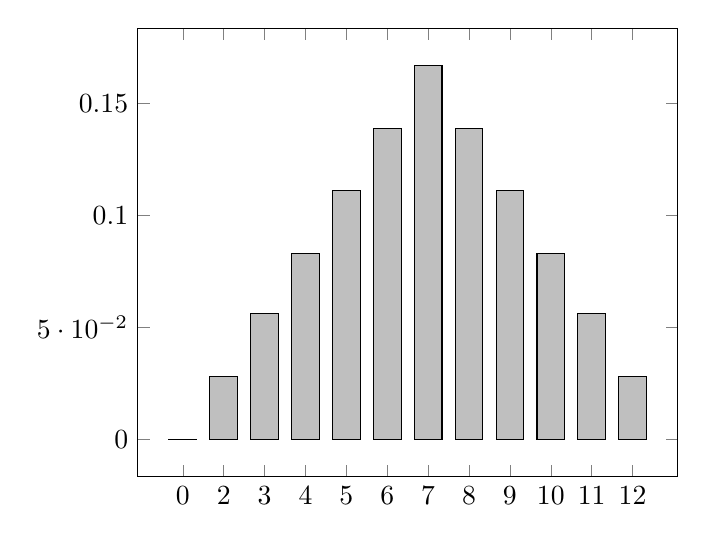
\begin{tikzpicture}
        \begin{axis}[
            symbolic x coords={0, 2, 3, 4, 5, 6, 7, 8, 9, 10, 11, 12},
            xtick=data
          ]
            \addplot[ybar,fill=lightgray] coordinates {
                (0, 0.0000001)
                (2, 0.028)
                (3,  0.056)
                (4,   0.083)
                (5,   0.111)
                (6,  0.139)
                (7,   0.167)
                (8,   0.139)
                (9,  0.111)
                (10,   0.083)
                (11,   0.056)
                (12,  0.028)
            };
        \end{axis}
    \end{tikzpicture}
    

\begin{tikzpicture}
\begin{axis}
\addplot+[ycomb, color=black] plot coordinates
	{(0,3) (1,2) (2,4) (3,1) (4,2)};
\end{axis}
\end{tikzpicture}

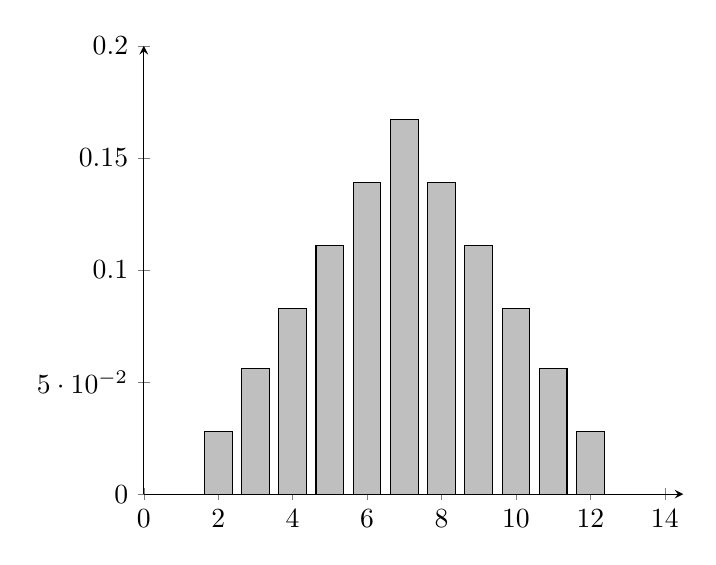
\begin{tikzpicture}
\begin{axis}[axis x line=bottom,
	axis y line=left, ymax=0.2, ymin=0, xmax=14.5, xmin=0]
\addplot [ybar, color=black, fill=lightgray] coordinates
	{           (0, 0)
	            (1, 0)
                (2, 0.028)
                (3,  0.056)
                (4,   0.083)
                (5,   0.111)
                (6,  0.139)
                (7,   0.167)
                (8,   0.139)
                (9,  0.111)
                (10,   0.083)
                (11,   0.056)
                (12,  0.028)}
                (13, 0)
                (14, 0);
\end{axis}
\end{tikzpicture}

% \begin{align*}
%     % p_X(2)=\frac{1}{36}; \quad  p_X(3)=\frac{2}{36}; \quad p_X(4)=\frac{3}{36}; \quad  p_X(5)=\frac{4}{36}; \quad
%     % p_X(6)=\frac{5}{36}\\
%     % p_X(7)=\frac{6}{36}\\
%     % p_X(8)=\frac{5}{36}\\
%     % p_X(9)=\frac{4}{36}\\
%     % p_X(10)=\frac{3}{36}\\
%     % p_X(11)=\frac{2}{36}\\
%     % p_X(12)=\frac{1}{36}\\
% \end{align*}

\end{eks}

%$\Sigma = {{}, {1}, {2}, {3}, {4}, {5}, {6}, {1, 2}, {1, 3}, {1, 4}, {1, 5}, {1, 6}, {2, 3}, {2, 4}, {2, 5}, {2, 6}, {3, 4}, {3, 5}, {3, 6}, {4, 5}, {4, 6}, {5, 6}, {1, 2, 3}, {1, 2, 4}, {1, 2, 5}, {1, 2, 6}, {1, 3, 4}, {1, 3, 5}, {1, 3, 6}, {1, 4, 5}, {1, 4, 6}, {1, 5, 6}, {2, 3, 4}, {2, 3, 5}, {2, 3, 6}, {2, 4, 5}, {2, 4, 6}, {2, 5, 6}, {3, 4, 5}, {3, 4, 6}, {3, 5, 6}, {4, 5, 6}, {1, 2, 3, 4}, {1, 2, 3, 5}, {1, 2, 3, 6}, {1, 2, 4, 5}, {1, 2, 4, 6}, {1, 2, 5, 6}, {1, 3, 4, 5}, {1, 3, 4, 6}, {1, 3, 5, 6}, {1, 4, 5, 6}, {2, 3, 4, 5}, {2, 3, 4, 6}, {2, 3, 5, 6}, {2, 4, 5, 6}, {3, 4, 5, 6}, {1, 2, 3, 4, 5}, {1, 2, 3, 4, 6}, {1, 2, 3, 5, 6}, {1, 2, 4, 5, 6}, {1, 3, 4, 5, 6}, {2, 3, 4, 5, 6}, {1, 2, 3, 4, 5, 6}}$

\textit{Indtil videre} har hændelsen været på formen $\{X=k\}$, hvor $X$ har antaget én bestemt værdi, $k$. Dette kan udvides til hændelser på formen $\{X\leq k\}$, hvor $X$ antager værdier mindre eller lig $k$. Dette kan defineres som følgende funktion

\begin{minipage}\textwidth
\begin{defn}\textbf{Kumulative fordelingsfunktion} %Ny definition
\newline
Lad $X$ være en tilfældig variabel. Funktionen 
$$F(x)=P(X\leq x), \quad x\in\R$$
kaldes for den kumulative fordelingsfunktion (cdf) af $X$
\end{defn}
\end{minipage}

%A real random variable is a real valued function from the possible outcome of a random experiment.

\begin{minipage}\textwidth
\begin{pro} \textbf{} %Ny proposition
\newline
Lad $X$ være en diskret tilfældig variabel med $range(X)=\{x_k | k\in N \subseteq \N\}$, frekvensfunktion, $p$, og kumulative fordelingsfunktion, $F$. Så gælder det, at
\begin{enumerate}
    \item $\displaystyle F(x)=\displaystyle\sum_{k:x_k\leq x}p(x_k), \quad x\in\R$
    \item $\displaystyle p(x_k)=F(x_k)-\lim_{y\uparrow x_k} F(y), \quad k=1, 2,\cdots$
    \item For $B\subseteq \R$, $\displaystyle P(X\in B)=\displaystyle\sum_{k:x_k\in B}p(x_k)$
\end{enumerate}
\end{pro}
\end{minipage}

%\section{Fordelinger - Mikkel}
%\input{Afsnit/Sandsynlighed/Fordelinger}

\section{Forventet værdi og varians}



%\textit{Den forventede værdi} afhænger af de gennemsnitlige værdier af et eksperiment. 
Ud fra frekvensfunktionen, er det muligt at bestemme den \textit{forventede værdi} for en diskret tilfældig variabel. Den forventede værdi afhænger af de gennemsnitlige værdier for de diskrete tilfældige variabler i et tilfældigt eksperiment, $\E$. Den forventede værdi defineres som følgende.

\begin{minipage}\textwidth
\begin{defn}\textbf{Forventet værdi} \label{def:Forventetværdi} %Ny definition 
\newline
Lad $X$ være en diskret tilfældig variabel med den tilhørende frekvensfunktion $p_X$. Den forventede værdi af $X$ er defineret ved
\begin{align}
E[X]=\sum_{x\in \text{Range}(X)} x p_X(x),
\end{align}
hvis summen er absolut konvergent.
\end{defn}
\end{minipage}

Den forventede værdi er et vægtet gennemsnit af de mulige værdier af $X$ med tilsvarende sandsynligheder som vægte. 

Den forventede værdi af en funktion, som afhænger af $X$, kan opstilles som følgende

\begin{minipage}\textwidth
\begin{pro} \textbf{} \label{prop:forventet_værdi_af_funktion} %Ny proposition
\newline
Lad $X$ være en diskret tilfældig variabel med den tilhørende frekvensfunktion $p_X$. Lad $g: \R \to \R$ være en reel funktion. Så gælder det, at
\begin{align}           
    E\left[g(X)\right]=\sum_{x \in \text{Range}(X)} g(x)p_X(x),
\end{align}
hvis summen er absolut konvergent.
\end{pro}
\end{minipage}

\begin{bev}\textbf{} %Nyt bevis
\newline
Lad $(\Omega, \F, P)$ være et sandsynlighedsrum og $X: \Omega \to \R$ være en diskret tilfældig variabel med frekvensfunktion, $p_X$. Lad $I= \text{Range}(X)$ og $Y=g(X)$, så er $Y$ en diskret tilfældig variabel med billede $\text{Range}\hspace{-2pt}\left(g(I)\right)$ og den tilhørende frekvensfunktion $p_Y$. Fra \autoref{def:Frekvensfunktionen} og \autoref{def:Diskret_tilfældig_variabel} gælder det, at
%
\begin{align*}
    p_Y(y) = P(Y = y) = P\left(\{\omega \in \Omega: Y(\omega) = y\}\right).
\end{align*}
%
Af \autoref{def:Forventetværdi} følger det, at
%
\begin{align}\label{eq:E[Y]}
    E[Y] = \sum_{y \in \text{Range}\left(g(I)\right)} yp_Y(y).
\end{align}
%
For ethvert $y\in \text{Range}\hspace{-2pt}\left(g(I)\right)$ eksisterer der mindst et $x\in I$ således, at $g(x)=y$. Dette medfører, at
% 
\begin{align*}
    P\left(\{\omega \in \Omega: Y(\omega) = y\}\right) = P\left(\left\{\omega \in \Omega: X(\omega) \in \{x\in I| g(x)=y\}\right\}\right).
\end{align*}
Derudover gælder det, at
\begin{align*}
    \left\{\omega \in \Omega: X(\omega) \in \{x\in I| g(x)=y\}\right\} = \bigcup_{\substack{x \in I:\\ g(x) =y}} \{\omega \in \Omega |X(\omega) = x\}.
\end{align*}
Hvorom det gælder, at
\begin{align*}
    \{\omega \in \Omega | X(\omega)=x_j\} \cap \{\omega \in \Omega | X(\omega)=x_i\} = \emptyset \text{ for alle } i,j=1,2, \ldots \Rightarrow x_j\neq x_i.
\end{align*}
Det følger da af \autoref{def:ovegangsmatrice} punkt 3 og \autoref{def:Frekvensfunktionen}, at
\begin{align}
    P\left(\left\{\omega \in \Omega: X(\omega) \in \{x\in I| g(x)=y\}\right\}\right)&=\sum_{\substack{x \in I:\\ g(x) =y}} P\left(\{\omega \in \Omega |X(\omega) = x\}\right)\nonumber\\
    &=\sum_{\substack{x \in I:\\ g(x) =y}}p_X(x).\label{eq:bevis_for_forventet_værdi_som_funktion_2}
\intertext{Ved at indsætte \eqref{eq:bevis_for_forventet_værdi_som_funktion_2} i \eqref{eq:E[Y]} fås følgende}
    E[Y] = \sum_{y \in \text{Range}\left(g(I)\right)} y\left( \sum_{\substack{x \in I:\\ g(x) =y}}p_X(x) \right)
    &=\sum_{y \in \text{Range}\left(g(I)\right)}\sum_{\substack{x \in I:\\ g(x) =y}} g(x) p_X(x). \nonumber\\
    \intertext{Da}
    \bigcup_{y\in \text{Range}\left(g(I)\right)}\bigcup_{\substack{x\in I\\g(x)=y}}\{x\}&=\bigcup_{y\in\text{Range}\left(g(I)\right)}\{x\in I|g(x)=y\} = I,\nonumber\\
    \intertext{følger det, at}
    \sum_{y \in \text{Range}\left(g(I)\right)}\sum_{\substack{x \in I:\\ g(x) =y}} g(x) p_X(x)&=\sum_{x\in I}g(x)p_X(x). \nonumber
\end{align}

Da $Y=g(X)$ og $I = \text{Range}(X)$, gælder det, at
\begin{align*}
    E\left[g(X)\right]=\sum_{x\in \text{Range}(X)}g(x)p_X(x).
\end{align*}
Dermed er \autoref{prop:forventet_værdi_af_funktion} bevist.
\end{bev}

Hvis sandsynligheden for en diskret tilfældig variabel, $X$, er betinget af en hændelse, $B\in\F$, påvirker det sandsynlighedsfordelingen af $X$. Sandsynligheden $P(X=x)$ erstattes derfor af $P(X=x|B)$.

\begin{minipage}\textwidth
\begin{defn}\textbf{Betingede forventede værdi}\label{def:betinget_forventet_værdi} %Ny definition
\newline
Lad $(\Omega, \F, P)$ være et sandsynlighedsrum og $B\in\F$ en hændelse. Lad $X$ være en diskret tilfældig variabel og $P(B)>0$. Så er den betingede forventede værdi af $X$ givet $B$ defineret ved 
\begin{align*}
    E[X|B]&=\sum_{x\in Range(X)}xP(X=x|B),
\end{align*}
hvis summen er absolut konvergent.
\end{defn}
\end{minipage}

I ovenstående definition er den forventede værdi af den diskrete tilfældige variabel, $X$, betinget af en hændelse, $B$. Hvis den forventede værdi af en diskret tilfældig variabel $X$ derimod er betinget af udfaldet af en anden diskret tilfældig variabel $Y$, defineres den betingede forventede værdi som følgende

\begin{minipage}\textwidth
\begin{defn}\textbf{Betingede forventede værdi af en diskret tilfældig variabel}\label{def:betinget_forventet_værdi_af_diskrete_tilfældige_variabler} %Ny definition
\newline
Lad $X, Y$ være diskrete tilfældige variabler. Så er den betingede forventede værdi af $X$ givet $Y$, givet ved
\begin{align*}
    E[X|Y=y] = \sum_{x\in Range(X)}xP(X=x|Y=y),
\end{align*}
hvis summen er absolut konvergent.
\end{defn}
\end{minipage}

Den forventede værdi giver ikke information om variationen for $X$. Derfor introduceres begrebet \textit{varians}, hvilket defineres som følgende

\begin{minipage}\textwidth
\begin{defn}\textbf{Varians}\label{def:varians} %Ny definition
\newline
Lad $X$ være en diskret tilfældig variabel med den forventede værdi, $E[X]$. Så er variansen af $X$ givet ved
\begin{align*}
    \text{Var}[X]=E\left[\left(X-E[X]\right)^2\right].
\end{align*}
\end{defn}
\end{minipage}

%Fremadrettet beskrives varians ved $\sigma^2$. 

%Jo større variansen er jo mere varierer X omkring den forventede værdi.

Bemærk desuden, at variansen er større end eller lig $0$. En højere varians medfører en større gennemsnitlig afvigelse fra den forventede værdi. Dette kaldes også for \textit{standardafvigelse}, som præsenteres i følgende definition.

\begin{minipage}\textwidth
\begin{defn}\label{def:standardafvigelse}\textbf{Standardafvigelse} %Ny definition
\newline
Lad $X$ være en diskret tilfældig variabel med varians, $\text{Var}[X]$. Standardafvigelsen for $X$ er defineret ved
$$\sigma = \sqrt{\text{Var}[X]}.$$
\end{defn}
\end{minipage}

Følgende korollar kan i nogle tilfælde simplificere beregningen af variansen.

\begin{minipage}\textwidth
\begin{kor} \textbf{}\label{kor:varians} %Nyt korollar
\newline
Lad $X$ være en diskret tilfældig variabel med den forventede værdi, $E[X]$. Så er variansen givet ved
\begin{align*}
    \text{Var}[X]=E[X^2] - \left(E[X]\right)^2.
\end{align*}
\end{kor}
\end{minipage}

\begin{bev} \textbf{} %Nyt bevis
\newline
Lad $X$ være en diskret tilfældig variabel med den tilhørende frekvensfunktion, $p_X$, og lad $I=\text{Range}(X)$. Det følger af \autoref{def:varians} og \autoref{prop:forventet_værdi_af_funktion}, at
\begin{align*}
    \text{Var}[X] &=E\left[\left(X-E[X]\right)^2\right] \\
    &=\sum_{x\in I}\left(x-E[X]\right)^2 p_X(x)\\
    &= \sum_{x\in I} \left(x^2-2xE[X]+\left(E[X]\right)^2\right)p_X(x)\\
    &= \sum_{x\in I} x^2p_X(x) - 2E[X] \sum_{x\in I} x p_X(x) + \left(E[X]\right)^2 \sum_{x\in I} p_X(x)\\
    &= E[X^2]-2\left(E[X]\right)^2+\left(E[X]\right)^2
    = E[X^2] - \left(E[X]\right)^2.
\end{align*}
Dermed er \autoref{kor:varians} bevist.
\end{bev}

Den forventede værdi og varians af et terningkast beregnes i \autoref{eks:forv_og_var}.

\begin{eks} \textbf{} \label{eks:forv_og_var} %Nyt eksempel
\newline
Lad $\E$ være et tilfældigt eksperiment hvor der kastes en fair terning. Lad $X$ være en tilfældigt variabel til $\E$ med tilhørende frekvensfunktion $p_X$.

%Hvis frekvensfunktionen har den samme værdi for alle mulige udfald, siges mængden af sandsynligheder at væreuniform fordelt.

Frekvensfunktionen er uniformt fordelt med $\text{Range}(X)=\{1,2,3,4,5,6\}$ og $p_X=\frac{1}{6}$.
Dermed er den forventede værdi givet ved
\begin{align*}
    E[X]=\sum_{x=1}^6 xp_X(x) = \dfrac{1}{6}\sum_{x=1}^6 x=\dfrac{7}{2}.
\end{align*}
Ved brug af \autoref{prop:forventet_værdi_af_funktion} fås
\begin{align*}
    E[X^2]=\sum_{x=1}^6  x^2 p_X(x) = \dfrac{1}{6} \sum_{x=1}^6 x^2 = \dfrac{91}{6}.
\end{align*}
Ud fra \autoref{kor:varians} bestemmes variansen
\begin{align*}
    \text{Var}[X]  &=E[X^2]-\left(E[X]\right)^2\\
            &=\frac{91}{6} - \left(\frac{7}{2}\right)^2 = \dfrac{35}{12}.
\end{align*}
Dermed er variansen for et terningkast bestemt til at være $\text{Var}[X] = \displaystyle \frac{35}{12}$ og den forventede værdi er $\frac{7}{2}$.
\end{eks}



%\section{Betinget forventet værdi}
%%I ovenstående afsnit gælder resultaterne for én diskret tilfældig variabel. Dette kan udvides til \textit{diskrete tilfældige vektorer}.

%\begin{minipage}\textwidth
%\begin{defn}\textbf{Diskret tilfældig vektor} %\label{def:fælles_frekvensfunktion}%Ny %definition
%\newline
%Lad $X_1, X_2, \dots, X_n$ være diskrete %tilfældige variabler, så gælder det at $(X_1, %X_2, \dots, X_n)$ kaldes en n-dimensional %diskret tilfældig vektor.
%\end{defn}
%\end{minipage}
%$\{(x_i,x_j\cdots x_k) for i,j,k=1, 2...n\}$
%....

%\begin{minipage}\textwidth
%\begin{defn}\textbf{Fælles frekvensfunktion} %\label{def:fælles_frekvensfunktion}%Ny %definition
%\newline
%Lad $X_1, X_2, \dots, X_n$ være diskrete %tilfældige variabler på sandsynlighedsrummet %$(\omega, \mathcal{F}, P)$. Funktionen $p_{X_1, %X_2, \dots, X_n}:\R^n\to [0, 1]$ defineret ved 
%\begin{align*}
%    p_{X_1, X_2, \dots, X_n}(x_1, x_2, \dots, %x_n)=P(X_1=x_1, X_2=x_2, \dots, X_n=x_n)
%\end{align*}
%kaldes for en \textit{fælles frekvensfunktion} %eller \textit{fælles pmf} til $(X_1, X_2, %\dots, X_n)$.
%\end{defn}
%\end{minipage}




